\documentclass{beamer}
\usetheme[pageofpages=of,% String used between the current page and the
                         % total page count.
          bullet=circle,% Use circles instead of squares for bullets.
          titleline=true,% Show a line below the frame title.
          alternativetitlepage=true,% Use the fancy title page.
       %   titlepagelogo=logo-polito,% Logo for the first page.
       %   watermark=watermark-polito,% Watermark used in every page.
       %   watermarkheight=100px,% Height of the watermark.
       %   watermarkheightmult=4,% The watermark image is 4 times bigger
                                % than watermarkheight.
          ]{Torino}

\setbeamertemplate{footline}{
  \begin{beamercolorbox}[wd=\paperwidth,ht=1ex,dp=1ex]{footline}
    \vspace{5pt} \hspace{1em} \insertframenumber/\inserttotalframenumber
  \end{beamercolorbox}
}

\author{Brendon J. Brewer}
\title{STATS 331 -- Introduction to Bayesian Statistics}
\institute{The University of Auckland}
\date{}


\linespread{1.3}
\usepackage{minted}
\usepackage[utf8]{inputenc}
\usepackage{dsfont}
\newcommand{\given}{\,|\,}

\begin{document}

\frame{\titlepage}

\begin{frame}
\begin{center}
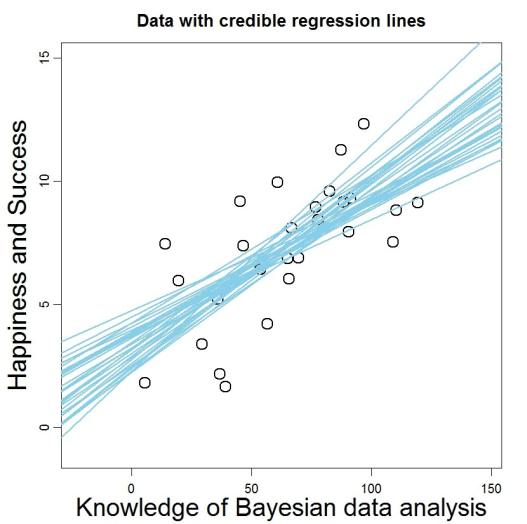
\includegraphics[width=0.6\textwidth]{images/happiness.png} \\
Credit: John Kruschke
\end{center}

\end{frame}


\begin{frame}
\frametitle{Plan}
\begin{itemize}
\item We will now look at two examples of Bayesian parameter estimation,
one of which also involves a {\bf prediction}.\pause
\item In both cases, we'll get the likelihood by defining the
{\bf sampling distribution} first.\pause
\item We will introduce a different ``non-informative'' prior distribution
that isn't uniform.
\end{itemize}

\end{frame}


\begin{frame}
\frametitle{Reminder of Bayes' Rule for Parameter Estimation}

\begin{align}
p(\theta \given x) &= \frac{p(\theta)p(x \given \theta)}{p(x)} \\
p(\theta \given x) &\propto p(\theta)p(x \given \theta) \\
\texttt{posterior} &\propto \texttt{prior} \times \texttt{likelihood}
\end{align}
(notation: $\theta$=parameter, $x$=data)

\end{frame}



\begin{frame}
\frametitle{Taxi Problem}

    \begin{columns} % Create two columns
        \column{0.5\textwidth} % Left column (50% width)

        \begin{itemize}
        \item You fall asleep in a foreign city.
        \item When you wake up in the morning, you see a taxi drive by,
              which says {\bf This is taxi number 42}.
        \item How many taxis are in the city?
        \end{itemize}

        \column{0.5\textwidth} % Right column (50% width)
        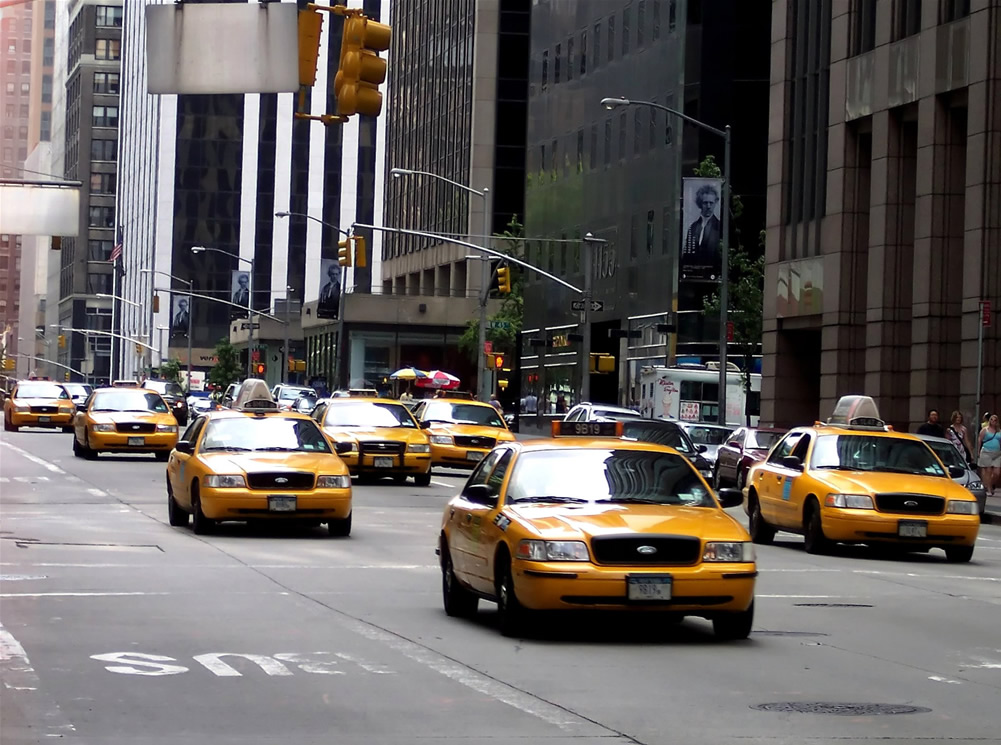
\includegraphics[width=0.95\linewidth]{images/taxis.jpg}
       
         (public domain image)
     \end{columns}

\end{frame}

\begin{frame}
\frametitle{The Parameter and the Data}

\begin{itemize}
\item The unknown parameter, $N$, is the number of taxis in the city.\pause
\item The data, $x$, is the number observed on the taxi that drove past.
\end{itemize}
\pause
Bayes' rule for this circumstance:

\begin{align}
p(N \given x) \propto p(N)p(x \given N)
\end{align}
We have to choose the prior $p(N)$ and the likelihood $p(x \given N)$.

\end{frame}


\begin{frame}
\frametitle{Bayes Box with Uniform Prior}
Let's assume $N \leq 100$ and keep our uniform prior for now.

\centering
{\footnotesize
\begin{tabular}{|c|c|c|c|c|}
\hline
Parameter & Prior & Likelihood & Prior $\times$ Likelihood & Posterior \\
$N$  & $p(N)$ & $p(x \given N)$ & $p(N)p(x\given N)$ & $p(N\given x)$ \\
\hline
1 & 0.01 & & & \\
2 & 0.01  &  & & \\
... &... &... & ...&... \\
41 & 0.01 &  & & \\
42 & 0.01  &  & & \\
43 & 0.01 & & & \\
... &... &... & ...&... \\
99 & 0.01 & & & \\
100   & 0.01 & & & \\
\hline
Total & 1 & & & 1 \\
\hline
\end{tabular}
}

\end{frame}

\begin{frame}
\frametitle{Likelihoods: Direct Reasoning}

\begin{itemize}
\item If $N=1$, with what probability would we observe $x=42$? \pause
\item If $N=41$, with what probability would we observe $x=42$? \pause
\item If $N=42$, with what probability would we observe $x=42$? \pause
\item If $N=100$, with what probability would we observe $x=42$?
\end{itemize}

\end{frame}


\begin{frame}
\frametitle{Likelihoods}

\centering
{\footnotesize
\begin{tabular}{|c|c|c|c|c|}
\hline
Parameter & Prior & Likelihood & Prior $\times$ Likelihood & Posterior \\
$N$  & $p(N)$ & $p(x \given N)$ & $p(N)p(x\given N)$ & $p(N\given x)$ \\
\hline
1 & 0.01 & 0 & & \\
2 & 0.01  & 0  & & \\
... &... &... & ...&... \\
41 & 0.01 & 0 & & \\
42 & 0.01  & 1/42 & & \\
43 & 0.01 & 1/43 & & \\
... &... &... & ...&... \\
99 & 0.01 & 1/99 & & \\
100   & 0.01 & 1/100 & & \\
\hline
Total & 1 & & & 1 \\
\hline
\end{tabular}
}

\end{frame}


\begin{frame}
\frametitle{Likelihoods: from Sampling Distribution}
Imagine we did not know $x$ yet, but we did know $N$, the parameter.
We can assign a probability distribution for $x$ given $N$.
This would be a discrete uniform distribution, and we can write
\begin{align}
x \given N &\sim \textnormal{Uniform}(1, 2, ..., N).
\end{align}\pause

The formula for this probability distribution is
\begin{align}
p(x \given N) &= \left\{
                    \begin{array}{lr}
                    \frac{1}{N}, & x \in \{1, 2, ..., N\} \\
                    0          , & \textnormal{otherwise}.
                    \end{array}
                 \right.
\end{align}
\end{frame}

\begin{frame}
\frametitle{Likelihoods: from Sampling Distribution}
If we take the formula and interpret it as a function of $N$
with $x$ fixed at 42, it reads
\begin{align}
p(x \given N) &= \left\{
                    \begin{array}{lr}
                    \frac{1}{N}, & 42 \in \{1, 2, ..., N\} \\
                    0          , & \textnormal{otherwise}.
                    \end{array}
                 \right.
\end{align}
which is exactly the rule we `guessed' earlier.


\end{frame}

\begin{frame}
\frametitle{Likelihoods: from Sampling Distribution}
In general, we can think of data as being `drawn from'
some distribution\footnote{Philosophically I object, but it is a useful
starting point.}
with unknown parameter $\theta$, written as $p(x \given \theta)$.
This will be a formula involving both $x$ and $\theta$.
\pause

When $x$ is known value (plugged in) but $\theta$ isn't, $p(x \given \theta)$
is now a function of $\theta$ only --- the likelihood function.
You may have seen this in STATS 210 or other courses. If not, this is a
reasonable first place to learn about it.

\end{frame}


\begin{frame}
\frametitle{Likelihoods: from Sampling Distribution}
Since sampling distributions are conditional on $\theta$ but not on the
data $x$, they are kind of a prior but for the data instead of the parameter.

\end{frame}



\begin{frame}[fragile]
\frametitle{Calculating the Posterior in R}
This follows the standard recipe, but the likelihood is slightly trickier
than what we had before.
\begin{minted}{r}
N = seq(1, 100)
prior = rep(1/length(N), length(N))
lik = 1/N
lik[N < 42] = 0
h = prior*lik
Z = sum(h)
post = h/Z
plot(N, post, type="h")
\end{minted}

\end{frame}

\begin{frame}
\frametitle{Taxi Posterior}

\centering
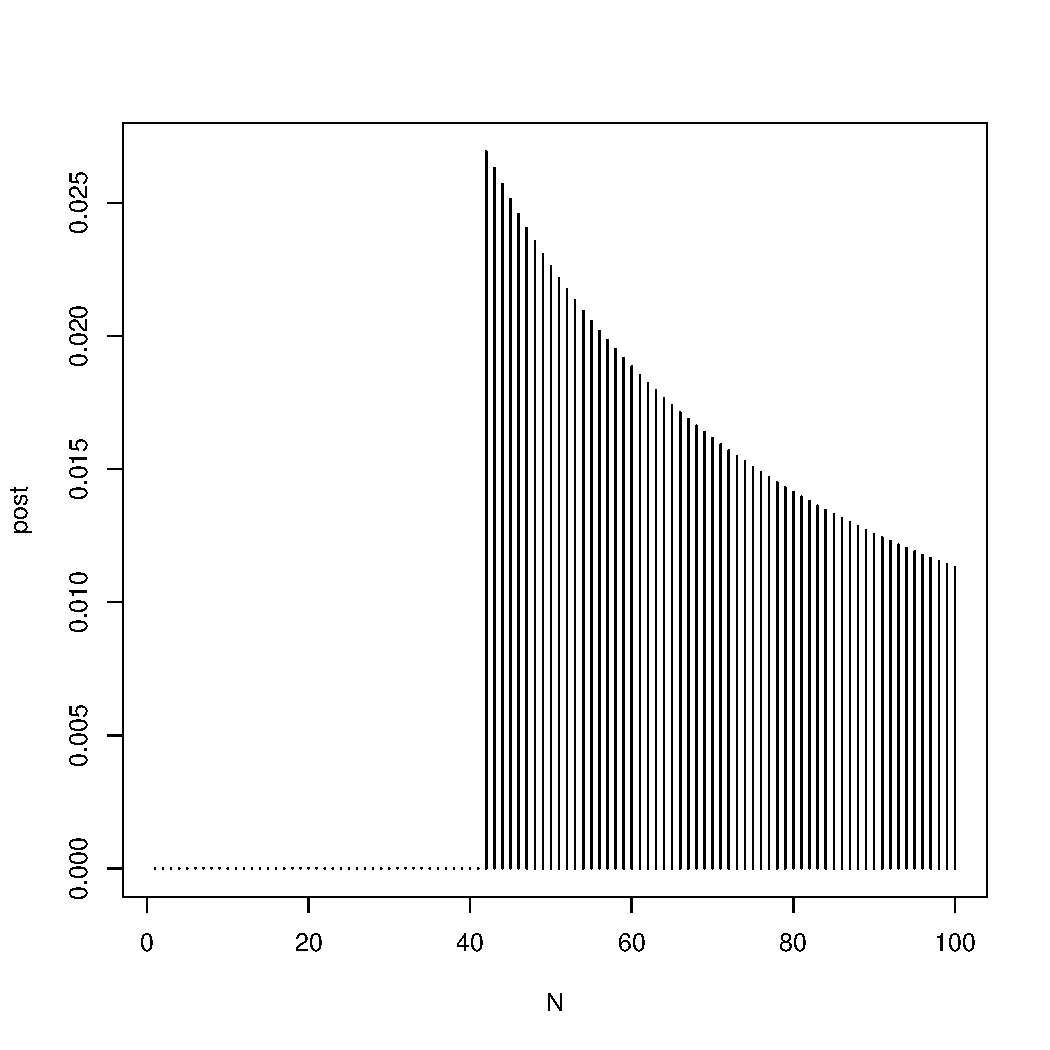
\includegraphics[width=0.6\textwidth]{images/taxi_posterior.pdf}

\end{frame}


\begin{frame}
\frametitle{Auckland Volcano Example}

\centering
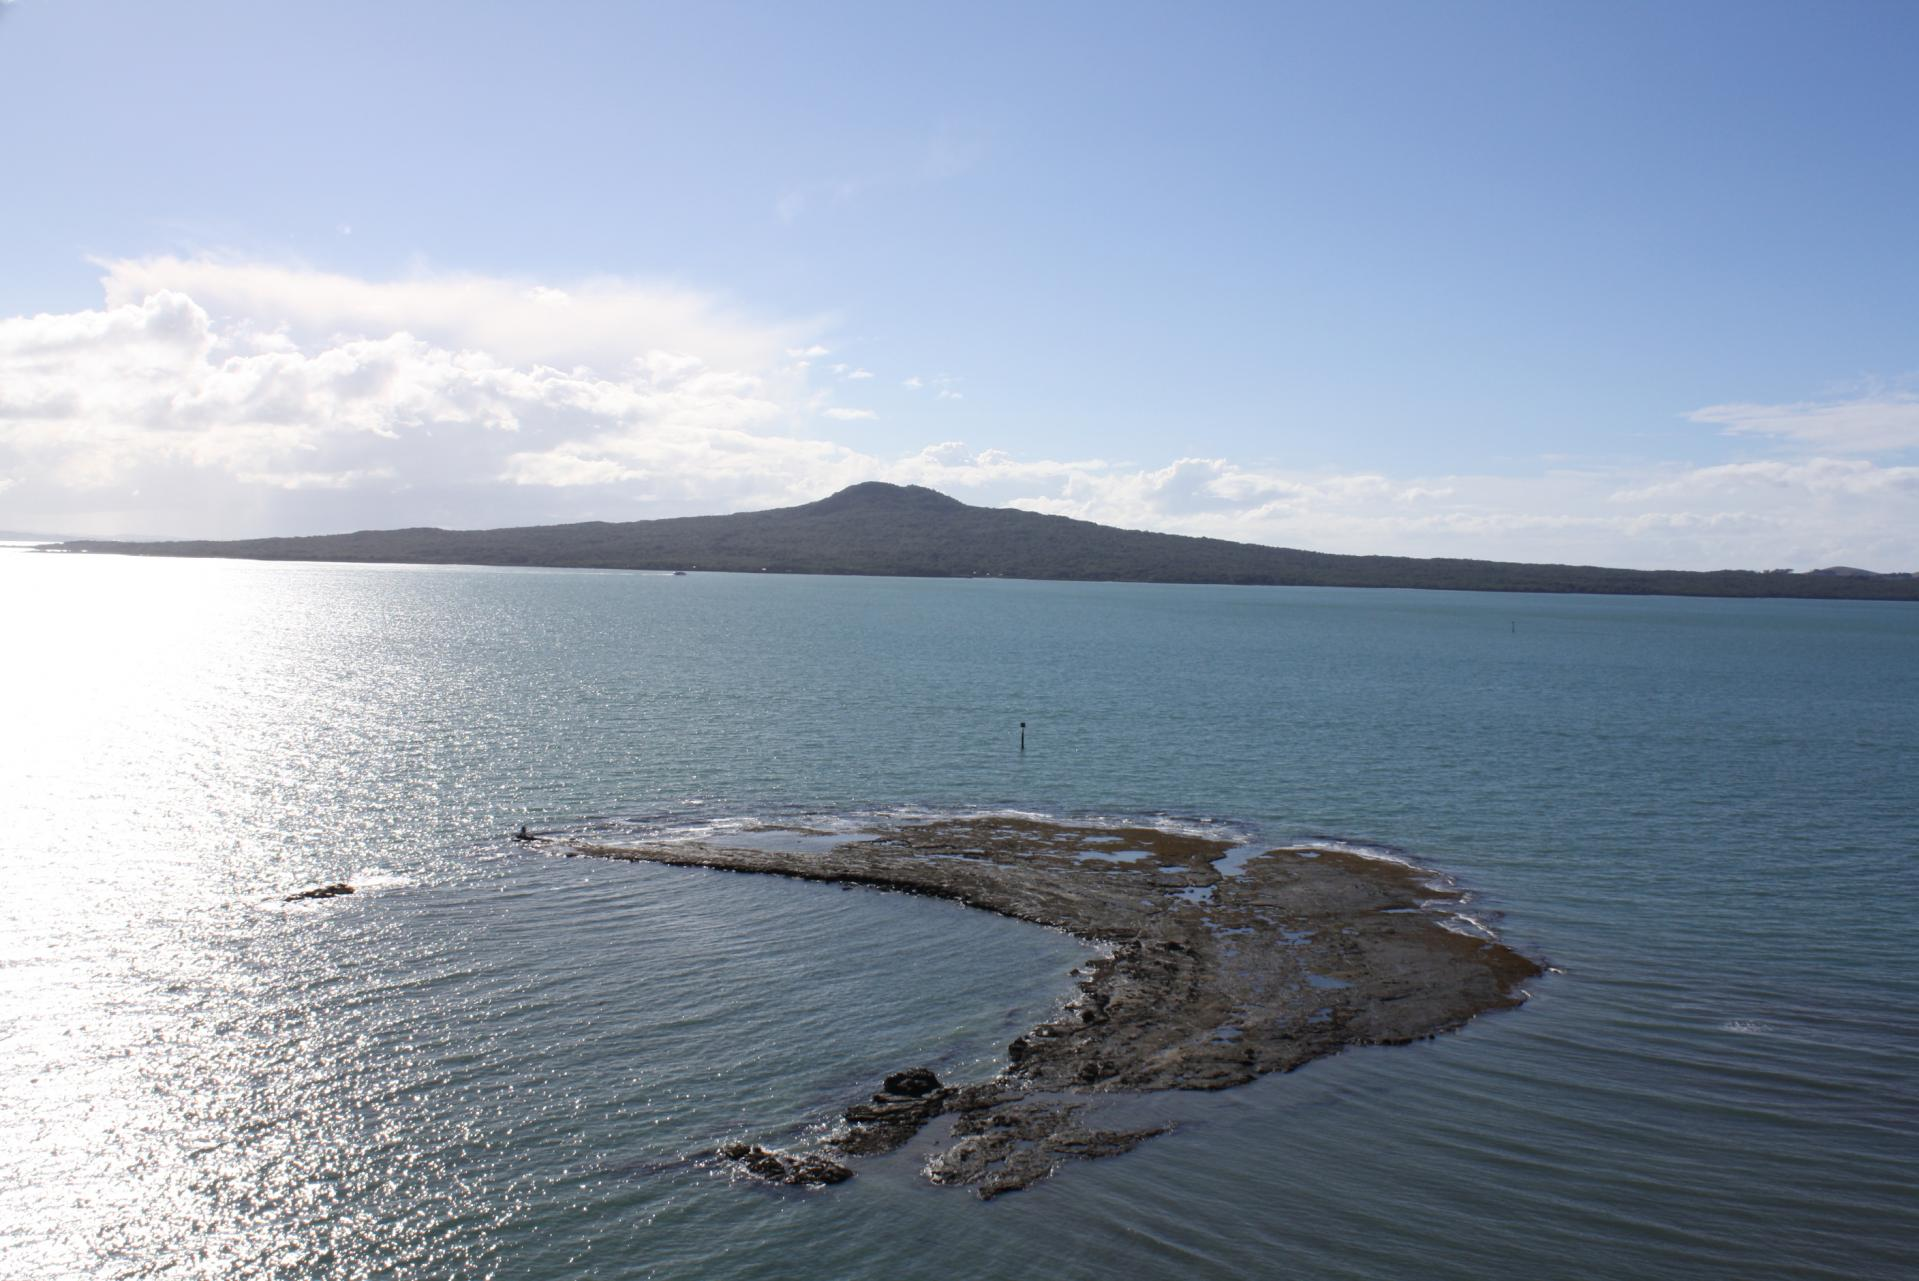
\includegraphics[width=0.7\textwidth]{images/rangitoto.jpg}

(public domain image)

\end{frame}



\begin{frame}
\frametitle{The Problem (based on STATS 210)}

\begin{itemize}
\item In the last 20,000 years, there have been 20 volcanic eruptions in the
Auckland region. Let's call this {\bf 1 time unit}.\pause
\item What is the probability of at least one eruption in the next 50 years
({\bf 0.0025 time units})?
\end{itemize}

\end{frame}


\begin{frame}[fragile]
\frametitle{Poisson Process}
Events occurring over time can be modelled using a ``Poisson Process''.
There is an average rate parameter $\lambda$.

\hspace{3em}
\begin{verbatim}
------*--*-----------*---------*--------------*--*-->
\end{verbatim}

\end{frame}


\begin{frame}
\frametitle{Poisson Process}
The number of events, $x$, in a time interval of length $t$ has a Poisson
distribution with mean $\lambda t$. We have an interval of unit length,
so we just get a Poisson with mean parameter $\lambda$:

\begin{align}
p(x \given \lambda) &= \frac{\lambda^x e^{-\lambda}}{x!}
\end{align}

\end{frame}


\begin{frame}
\frametitle{Poisson Process}
We could use the Poisson Process to get the probability
of an eruption in the next 50 years:
\begin{align}
P(\textnormal{Eruption} \given \lambda)
    &= 1 - e^{-0.0025\lambda}
\end{align}
(from the Poisson formula with mean $\lambda t$, evaluated at $x=0$).\\[1em]\pause

{\bf Problem}: We can't use this, because we don't know $\lambda$.
So let's do parameter estimation.


\end{frame}


\begin{frame}
\frametitle{Uniform Prior}

\centering
{\footnotesize
\begin{tabular}{|c|c|c|c|c|}
\hline
Parameter & Prior & Likelihood & Prior $\times$ Likelihood & Posterior \\
$\lambda$  & $p(\lambda)$ & $p(x \given \lambda)$ & $p(\lambda)p(x\given \lambda)$ & $p(\lambda\given x)$ \\
\hline
0.1 & 0.001 &  & & \\
1.1 & 0.001  &   & & \\
... &... &... & ...&... \\
19.9 & 0.001 &  & & \\
20.0 & 0.001  &  & & \\
20.1 & 0.001 &  & & \\
... &... &... & ...&... \\
99.9 & 0.001 &  & & \\
100.0   & 0.001 &  & & \\
\hline
Total & 1 & & & 1 \\
\hline
\end{tabular}
}

\end{frame}


\begin{frame}[fragile]
\frametitle{Likelihood}
We have a single data value $x=20$ `from a Poisson distribution' with unknown mean
$\lambda$. We could work with the Poisson formula, but it is easier to use
R's \mintinline{r}{dpois()} function.\pause

\begin{minted}{r}
lambda = seq(0.1, 100, by=0.1)
prior = rep(1/length(lambda), length(lambda))
lik = dpois(20, lambda)
\end{minted}
\pause

{\bf Note}: If you wanted to plot a Poisson distribution, you would use
\mintinline{r}{dpois()} with one value of $\lambda$ and a range of values
of $x$. Here we do the opposite because $x$ is known to be 20 and
$\lambda$ is unknown.
\end{frame}


\begin{frame}[fragile]
\frametitle{Computing and Plotting the Posterior}
\begin{minted}{r}
lambda = seq(0.1, 100, by=0.1)
prior = rep(1/length(lambda), length(lambda))
lik = dpois(20, lambda)
h = prior*lik
Z = sum(h)
post = h/Z
plot(lambda, post, type="h")
\end{minted}

\end{frame}



\begin{frame}[fragile]
\frametitle{Volcano Posterior Distribution}

\centering
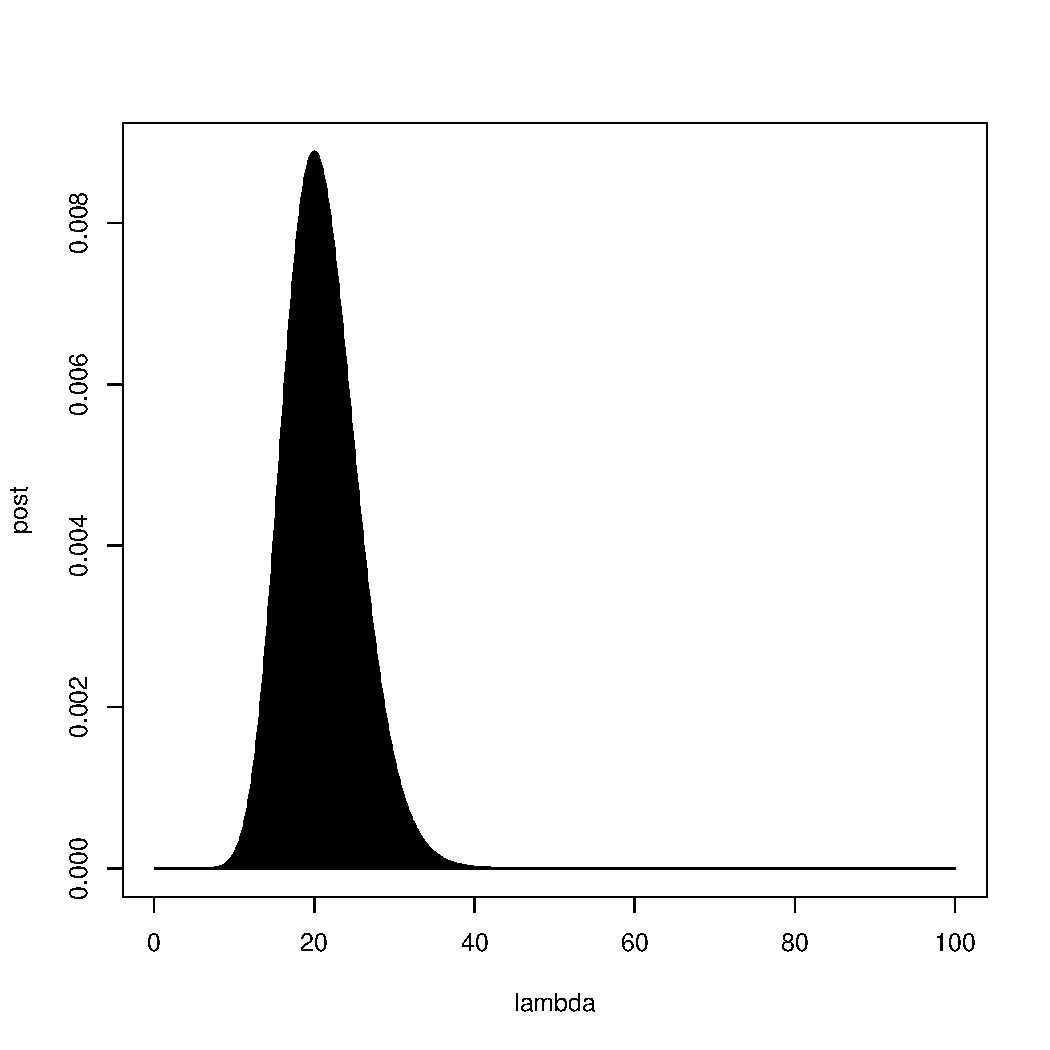
\includegraphics[width=0.6\textwidth]{images/volcano.pdf}

\end{frame}


\begin{frame}[fragile]
\frametitle{Volcano Posterior Distribution}

\begin{itemize}
\item The `maximum likelihood estimate' is at $\lambda=20$ for this problem.\pause
\item Since we used a uniform prior, this coincides with the peak of the
posterior distribution.\pause
\item The shape of the posterior distribution describes the uncertainty
about $\lambda$ completely.\pause
\item This is different from the frequentist approach, which
instead considers how
the maximum likelihood estimate would vary for different datasets.
\end{itemize}

\end{frame}


\begin{frame}
\frametitle{Another Prior: Log-Uniform}

\begin{itemize}
\item How long is a piece of string?\pause
\item Twice the distance from the middle to the end.
\end{itemize}

\end{frame}


\begin{frame}
\frametitle{The Log-Uniform Prior}
This is useful for a parameter $\theta$ in the situation where:

\begin{itemize}
\item $\theta$ is known to be positive.\pause
\item $\theta$ is unknown by orders of magnitude.\pause
\end{itemize}
\vspace{0.5em}
e.g., the distance to some astronomical object might be
$10^{11}$ metres, or maybe $10^{12}$ metres, or maybe $10^{13}$
metres. A uniform prior would be inappropriate here.

\end{frame}



\begin{frame}[fragile]
\frametitle{The Log-Uniform Prior Formula}

The formula for the log-uniform prior is
\begin{align}
p(\theta) &\propto \frac{1}{\theta}
\end{align}

It also corresponds to a uniform prior for $\log(\theta)$.
To construct one in R:
\begin{minted}{r}
theta = seq(0.01, 100, by=0.1) # Cannot include zero!
prior = 1/theta                # The prior shape 
prior = prior/sum(prior)       # Normalise
\end{minted}

\end{frame}



\begin{frame}[fragile]
\frametitle{Volcano Posterior: Log-Uniform Prior}

\centering
\includegraphics[width=0.6\textwidth]{images/volcano_posterior_comparison.pdf}


\end{frame}


\begin{frame}[fragile]
\frametitle{Volcano Posterior: Log-Uniform Prior}

\begin{itemize}
\item The posterior distribution is moved slightly to the left by the log-uniform prior, compared to the uniform one.\pause
\item Usually, if the data gives us a fair bit of information, the prior
only has a slight effect on the posterior distribution.\pause
\item The prior can have a larger effect on the value of the
marginal likelihood, which
matters for some applications.
\end{itemize}

\end{frame}



\begin{frame}[fragile]
\frametitle{Prediction}

\begin{center}

\includegraphics[width=0.5\textwidth]{images/crystal_ball.jpg}
\end{center}
\end{frame}


\begin{frame}
\frametitle{Prediction: Classical Approach}

\begin{itemize}
\item Step 1: Get an estimate (single number guess of the parameter)\pause
\item Step 2: Make the prediction (probably using the sampling distribution),
assuming the estimate was correct.\pause
\item Step 3: Optionally, consider how the result would have varied if the data had
been different.
\end{itemize}

\end{frame}


\begin{frame}
\frametitle{Prediction: Bayesian Approach}

\begin{itemize}
\item Step 1: get the posterior distribution for the parameter(s)\pause
\item Step 2: For each possible value of the parameter, compute the probability
you're interested in (e.g., probability of an eruption in the next 50
years).\pause
\item Step 3: Calculate the weighted average of the probabilities from the previous
step, using the posterior distribution for the weights.
\end{itemize}

\end{frame}


\begin{frame}
\frametitle{Prediction: Bayesian Approach}
Consider all the `ways' in which there could be an eruption in the next 50 years:
\begin{itemize}
\item $\lambda=0.01$ and there is an eruption.\pause
\item $\lambda=0.02$ and there is an eruption.\pause
\item $\lambda=0.03$ and there is an eruption.\pause
\item And so on.
\end{itemize}
These are mutually exclusive so we can add up their probabilities.
Mathematically, it's the partition theorem.

\end{frame}

\begin{frame}[fragile]
\frametitle{The Two Results}

\begin{minted}{r}
# Classical
> 1 - dpois(0, 0.0025*20)
[1] 0.04877058

# Bayesian
> prob = 1 - dpois(0, 0.0025*lambda)
> sum(post*prob)
[1] 0.04871122
\end{minted}

\end{frame}

\begin{frame}[fragile]
\frametitle{The Two Results}
The results are numerically very similar.\\
{\bf Food for Thought}: When would you expect the two methods to give very
different results?

\end{frame}


\end{document}

